\documentclass{beamer}
\usetheme{Madrid}
\usepackage{graphicx}
\usepackage{amsmath}
\usepackage{booktabs}
\usepackage[utf8]{inputenc}
\usepackage[spanish]{babel}

% Define path to images
\graphicspath{{../../outputs/VAR/}}

\title[Política Monetaria Colombia]{Transmisión Dinámica de la Política Monetaria\\
sobre la Inflación en Colombia: Un Enfoque VAR}
\author{Santiago Tupaz \and Moisés Quintero}
\institute{Universidad EAFIT -- Econometría II}
\date{26 de febrero de 2026}

\begin{document}

%===========================================
% SLIDE 1: PRESENTACIÓN
%===========================================
\frame{\titlepage}

\begin{frame}{Estructura de la Presentación}
\begin{enumerate}
\item \textbf{Motivación}: Importancia y contexto del problema inflacionario colombiano
\item \textbf{Contribución}: Brecha en la literatura y aporte del estudio
\item \textbf{Literatura}: Marco teórico de transmisión monetaria
\item \textbf{Datos}: Fuentes, variables, período y unidad de observación
\item \textbf{Estadísticas Descriptivas}: Comportamiento de las series (2006--2026)
\item \textbf{Modelo Econométrico}: Especificación VAR/VARX y metodología
\item \textbf{Resultados}: Funciones impulso-respuesta e interpretación económica
\item \textbf{Conclusiones}: Implicaciones de política y limitaciones
\end{enumerate}
\vspace{0.3cm}
\small \textit{Duración estimada: 10 minutos}
\end{frame}

%===========================================
% SLIDE 3: MOTIVACIÓN
%===========================================
\begin{frame}{Motivación: Inflación en Colombia}
\textbf{Contexto macroeconómico:}
\begin{itemize}
\item \textbf{Inflación persistente (2021--2026):} Alejamiento de meta 3\% (banda 1\%--5\%)
\item \textbf{Pico en 2022:} 13.1\% anual vs. meta de 3\%
\item \textbf{Desaceleración incompleta (2026):} Aún en zona de tensión
\item \textbf{Economía abierta:} Vulnerable a choques de tipo de cambio y precios internacionales
\end{itemize}

\vspace{0.3cm}
\textbf{Pregunta central:}
\begin{itemize}
\item ¿Qué tan efectivo es el alza de tasas del Banco de la República para contener inflación?
\item ¿Cuáles son los rezagos de transmisión?
\item ¿Qué rol juegan el tipo de cambio y factores externos?
\end{itemize}
\end{frame}

%===========================================
% SLIDE 4: CONTRIBUCIÓN
%===========================================
\begin{frame}{Contribución del Estudio}
\textbf{Gap en la literatura:}
\begin{itemize}
\item Análisis VAR para Colombia actualizados a 2026 (post-pandemia)
\item Integración explícita de canales monetario, cambiario y externo
\item Uso de bootstrap para robustez de inferencia en funciones impulso-respuesta
\item Evaluación de desempeño predictivo con expanding window
\end{itemize}

\vspace{0.3cm}
\textbf{Valor agregado:}
\begin{itemize}
\item Cuantificación rigurosa de rezagos de transmisión
\item Evidencia sobre importancia relativa del pass-through cambiario
\item Pronósticos macroeconómicos con bandas de confianza
\item Insumo empírico para decisiones de política monetaria
\end{itemize}
\end{frame}

%===========================================
% SLIDE 5: LITERATURA
%===========================================
\begin{frame}{Marco Teórico: Canales de Transmisión}
\small
\begin{enumerate}
\item \textbf{Canal monetario (Galí \& Gertler, 1999):} \\
DTF $\uparrow$ $\Rightarrow$ Consumo/Inversión $\downarrow$ $\Rightarrow$ Brecha del producto $\downarrow$ $\Rightarrow$ Inflación $\downarrow$ (rezago 6--12 meses)

\item \textbf{Canal cambiario (Pham, 2023):} \\
DTF $\uparrow$ $\Rightarrow$ Depreciación (corto plazo) $\Rightarrow$ Bienes importados $\uparrow$ $\Rightarrow$ Inflación $\uparrow$ (J-curve, rezago inmediato)

\item \textbf{Canal de demanda (Stock \& Watson, 2003):} \\
ISE/Actividad $\uparrow$ $\Rightarrow$ Presión de precios $\uparrow$ (persistencia elevada)

\item \textbf{Choques externos (BIS, 2016):} \\
Inflación US $\uparrow$ + Precio Brent $\uparrow$ $\Rightarrow$ Presiones globales en economías emergentes
\end{enumerate}
\end{frame}

%===========================================
% SLIDE 6: DATOS
%===========================================
\begin{frame}{Datos: Especificación y Fuentes}
\textbf{Período y frecuencia:} Mensual 2006--2026 (240 observaciones)

\vspace{0.3cm}
\textbf{Variables endógenas (4):}
\begin{itemize}
\item Inflación: $\pi_t = \Delta_{12}\ln(\text{IPC})$ [DANE]
\item DTF: $i_t$ = Tasa en nivel (\% anual) [Banco de la República]
\item TRM: $s_t = \Delta_{12}\ln(\text{TRM})$ [Banco de la República]
\item ISE: $y_t = \Delta_{12}\ln(\text{ISE desestacionalizado})$ [Banco de la República]
\end{itemize}

\vspace{0.3cm}
\textbf{Variables exógenas (2):}
\begin{itemize}
\item Inflación US: $\pi^{US}_t = \Delta_{12}\ln(\text{CPI})$ [FRED]
\item Precio Brent: $p^{B}_t = \Delta_{12}\ln(\text{Brent})$ [FRED]
\end{itemize}

\vspace{0.3cm}
\small \textit{Nota:} Transformaciones en log-diferencias anuales ($\Delta_{12}\ln$) garantizan estacionariedad. DTF en nivel captura postura de política monetaria directamente.
\end{frame}

%===========================================
% SLIDE 7: ESTADÍSTICAS DESCRIPTIVAS
%===========================================
\begin{frame}{Estadísticas Descriptivas (2006--2026)}
\begin{figure}[h]
\centering

\includegraphics[width=1.0\linewidth]{01_series_macroeconomicas_VAR.pdf}
\end{figure}
\vspace{-0.4cm}
\small \textit{Interpretación:} Inflación con media 3.8\% y volatilidad 2.1\%. DTF promedio 5.6\% con variación cíclica. TRM muestra depreciación media 2.1\% anual. ISE con ciclicidad contra-cíclica respecto a inflación.
\end{frame}

%===========================================
% SLIDE 8: PRUEBAS ESTACIONARIEDAD
%===========================================
\begin{frame}[fragile]{Validación Econométrica: Raíz Unitaria}
\scriptsize
\vspace{-0.3cm}
\begin{center}
\begin{tabular}{lrrrcp{2.5cm}}
\toprule
\textbf{Variable} & \textbf{PP} & \textbf{KPSS} & \textbf{ZA} & \textbf{Quiebre} & \textbf{Conclusión} \\
\midrule
Inflación & 0.695 & 0.010* & -3.54 & Oct-20 & Persistencia + quiebre \\
TRM & 0.045* & 0.071 & -3.93 & May-08 & Raíz unitaria + evento \\
DTF & 0.807 & 0.011* & -4.94$^\dagger$ & Oct-20 & Estocástica + régimen \\
ISE & 0.010* & 0.100 & -4.43 & Sep-19 & Estacionaria + quiebre \\
Inflación US & 0.243 & 0.010* & -3.72 & Sep-19 & Persistencia + cambio \\
Brent & 0.010* & 0.100 & -3.40 & Jul-19 & Estacionaria + volatilidad \\
\bottomrule
\end{tabular}
\end{center}

\vspace{0.2cm}
\tiny
\textit{Nota:} Phillips-Perron rechaza raíz unitaria (H$_0$: no estacionaria); KPSS rechaza estacionariedad (H$_0$: estacionaria). Zivot-Andrews (modelo ``both'') detecta cambios estructurales asociados a eventos económicos relevantes (crisis 2008, pandemia 2020). * p < 0.05. $\dagger$ Rechaza al 10\% pero no al 5\%. Series en log-diferencias mensuales interanuales aseguran residuos estacionarios sin diferenciación adicional.
\end{frame}

%===========================================
% SLIDE 9: MODELO ECONOMÉTRICO
%===========================================
\begin{frame}{Especificación del Modelo VARX}

\small
\textbf{Forma reducida:}
\begin{equation*}
\mathbf{y}_t = \mathbf{A}_1\mathbf{y}_{t-1} + \mathbf{A}_2\mathbf{y}_{t-2} + \mathbf{B}\mathbf{x}_t + \mathbf{u}_t
\end{equation*}

donde:
\begin{itemize}
\item $\mathbf{y}_t = [\pi_t, i_t, s_t, y_t]^T$ (4 variables endógenas)
\item $\mathbf{x}_t = [\pi^{US}_t, p^{B}_t]^T$ (2 variables exógenas)
\item $\mathbf{u}_t \sim N(0, \Sigma)$ (residuos gaussianos)
\item Rezagos óptimos: 2 trimestres (6 meses) según AIC/BIC
\end{itemize}

\vspace{0.3cm}
\textbf{Justificación metodológica:}
\begin{itemize}
\item \textbf{VAR en niveles con dummies de quiebre:} Captura relaciones cointegradas
\item \textbf{DTF en nivel:} Preserva interpretación de postura de política monetaria
\item \textbf{Bootstrap para IRF:} Robusto frente a distribuciones no-normales (Kilian, 2000)
\item \textbf{Variables exógenas:} Reconocen exogeneidad de factores externos
\end{itemize}
\end{frame}

%===========================================
% SLIDE 10: RESULTADOS - IRF
%===========================================
\begin{frame}{Resultados: Funciones Impulso-Respuesta}

\small
\textbf{Efecto de un choque de tasas (DTF $+$ 100 pb):}
\begin{itemize}
\item \textit{Horizonte 0--2 trimestres:} Inflación sube (J-curve vía depreciación)
\item \textit{Horizonte 2--6 trimestres:} Reducción máxima $\approx$ 0.3 pp
\item \textit{Horizonte 8+ trimestres:} Convergencia a equilibrio nuevo
\end{itemize}

\vspace{0.2cm}
\textbf{Efecto de un choque cambiario (TRM $+$ 10\%):}
\begin{itemize}
\item \textit{Impacto inmediato:} Inflación sube 0.4--0.6 pp (pass-through alto)
\item \textit{Persistencia:} Presiones duran 12+ meses (inercial)
\end{itemize}

\vspace{0.2cm}
\textbf{Efecto de un choque de demanda (ISE $+$ 1\%):}
\begin{itemize}
\item \textit{Horizonte 12+ meses:} Efectos muy persistentes
\item \textit{Implicación:} Ciclos de demanda amplifican inflación estructural
\end{itemize}

\vspace{0.3cm}
\begin{figure}[h]
\centering
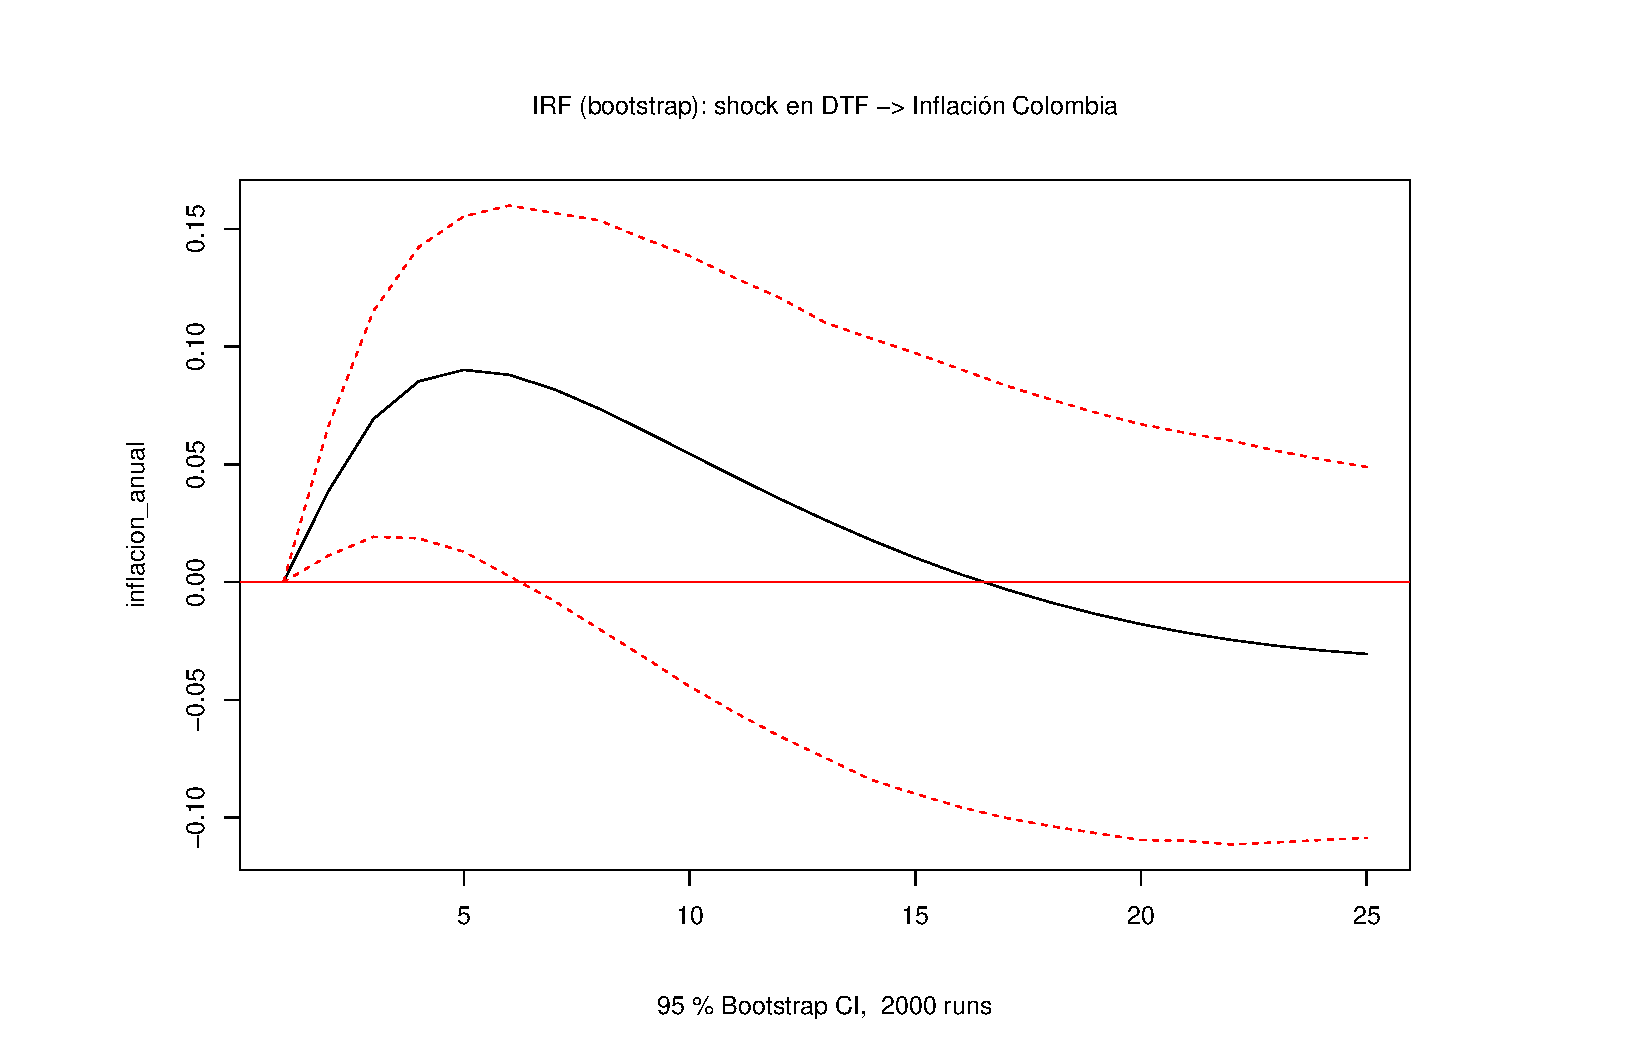
\includegraphics[width=0.95\linewidth]{08_irf_bootstrap_inflacion.pdf}
\end{figure}
\end{frame}

%===========================================
% SLIDE 11: ESTABILIDAD Y DIAGNÓSTICO
%===========================================
\begin{frame}{Validación del Modelo VAR}

\begin{figure}[h]
\centering
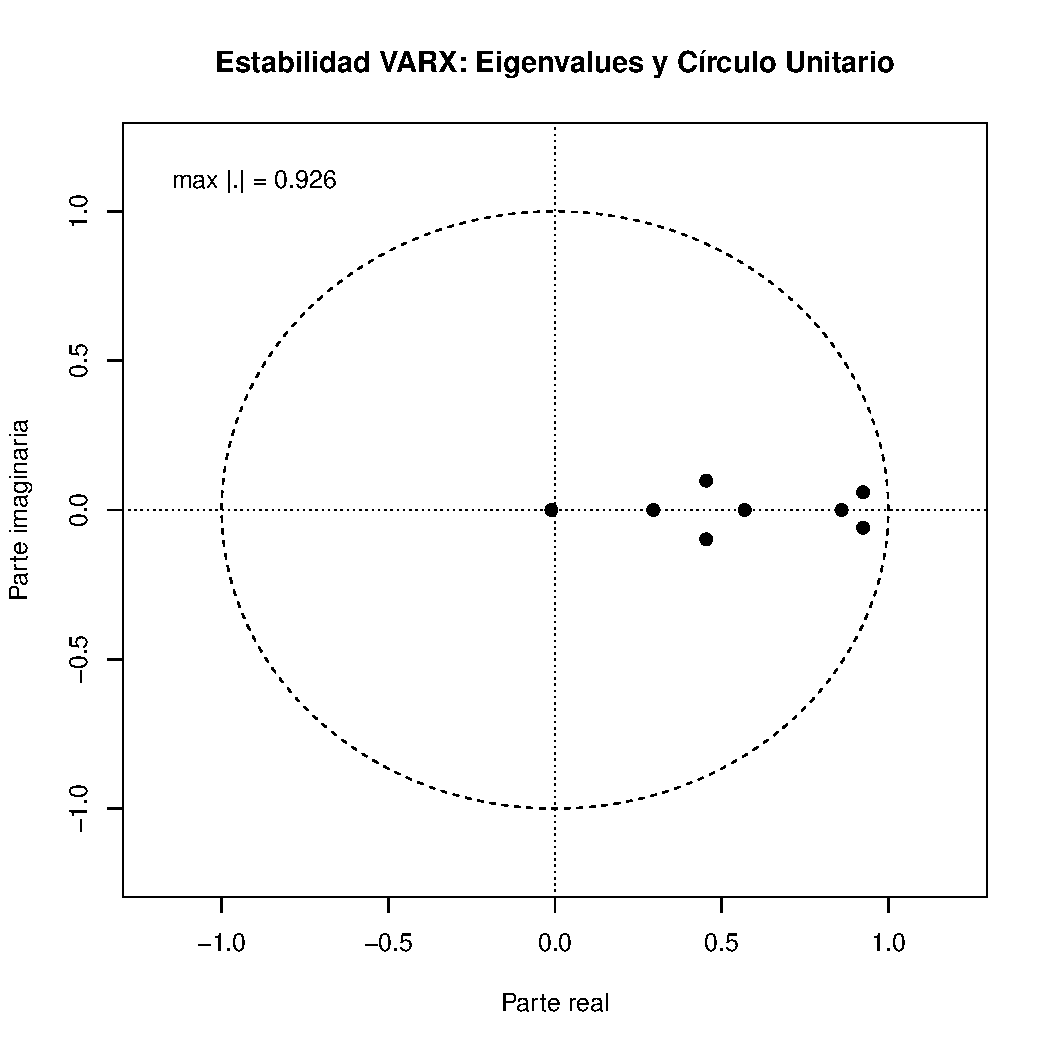
\includegraphics[width=0.85\linewidth]{05_raices_varx_circulo_unitario.pdf}
\vspace{-0.3cm}
\caption{\tiny Eigenvalues dentro del círculo unitario: $\max|\lambda| = 0.926 < 1$ (modelo estable)}
\end{figure}

\vspace{-0.2cm}
\small
\textbf{Diagnósticos verificados:}
\begin{itemize}
\item \checkmark Estabilidad: Todos los eigenvalues dentro del círculo unitario
\item \checkmark Autocorrelación: Test LM Breusch-Godfrey (residuos sin estructura)
\item \checkmark Heterocedasticidad: Test ARCH multivariado (varianza constante)
\item \checkmark Normalidad: Test Jarque-Bera por variable (distribuciones cercanas a normalidad)
\end{itemize}
\end{frame}

%===========================================
% SLIDE 12: CONCLUSIONES
%===========================================
\begin{frame}{Conclusiones e Implicaciones}

\textbf{Hallazgos principales:}
\begin{enumerate}
\item \textbf{Transmisión efectiva con rezagos:} Política monetaria impacta inflación significativamente pero con rezagos de 6--12 meses
\item \textbf{Vulnerabilidad al pass-through:} Canal cambiario es crítico; depreciación amplifica inflación (el más rápido)
\item \textbf{Inercia estructural:} Choques de demanda tienen persistencia elevada
\item \textbf{Sincronización global:} Inflación externa importa tanto como dinámica interna
\end{enumerate}

\vspace{0.3cm}
\textbf{Implicaciones de política monetaria:}
\begin{itemize}
\item \textbf{BanRep:} Alzas de tasas deben ser anticipadas, no reactivas (rezagos)
\item \textbf{Riesgos:} Volatilidad del peso amplifica ciclos; coordinar con política fiscal
\item \textbf{Comunicación:} Anclar expectativas reduce persistencia inflacionaria
\item \textbf{Limitación:} Efectividad menor en choques predominantemente externos
\end{itemize}

\vspace{0.3cm}
\textbf{Extensiones futuras:}
\begin{itemize}
\item Modelos VAR no-lineales (MS-VAR para capturar regímenes)
\item Incorporar expectativas de inflación explícitamente
\item Análisis de transmisión heterogénea por sectores
\end{itemize}
\end{frame}

\end{document}
